\documentclass[pdflatex,compress,mathserif]{beamer}

%\usetheme[dark,framenumber,totalframenumber]{ElektroITK}
\usetheme[darktitle,framenumber,totalframenumber]{ElektroITK}

\usepackage[utf8]{inputenc}
\usepackage[T1]{fontenc}
\usepackage{lmodern}
\usepackage[bahasai]{babel}
\usepackage{amsmath}
\usepackage{amsfonts}
\usepackage{amssymb}
\usepackage{graphicx}
\usepackage{multicol}
\usepackage{lipsum}

\newcommand*{\Scale}[2][4]{\scalebox{#1}{$#2$}}%

\title{METODE NUMERIK}
\subtitle{Interpolasi Polinom}

\author{Tim Dosen Pengampu}

\begin{document}

\maketitle

\section{Pengantar}

\begin{frame}
	\frametitle{Sub-CPMK dan Bahan Kajian}
	\begin{itemize}
		\item \textbf{Sub-CPMK:} Mahasiswa mampu menggunakan metode - metode interpolasi numerik
		\item \textbf{Bahan kajian:}
		\begin{enumerate}
			\item Interpolasi Polinom
			\item Polinom Lagrange
			\item Polinom Newton
			\item Polinom Newton-Gregory
			\item Interpolasi Dwimatra
		\end{enumerate}
	\end{itemize}
\end{frame}

\begin{frame}
	\frametitle{Pengantar}
	\begin{itemize}
		\item Sebuah pengukuran fisika telah dilakukan untuk menentukan hubungan antara tegangan yang diberikan kepada baja tahan-karat dan waktu yang diperlukan hingga baja tersebut patah.
		\item Delapan nilai tegangan yang berbeda dicobakan, dan data yang dihasilkan adalah
		\begin{center}
			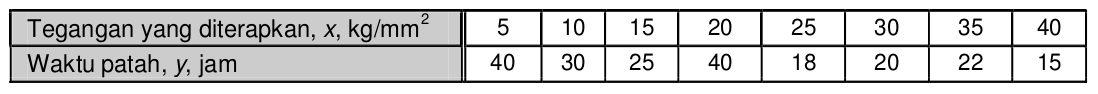
\includegraphics[width=\linewidth]{img/img01}
		\end{center}
		\item Berapa waktu patah $ y $ jika tegangan $ x $ yang diberikan kepada baja adalah 12 kg/mm$ ^2 $ .
	\end{itemize}
\end{frame}

\begin{frame}
	\begin{itemize}
		\item Solusinya dicari dengan metode pencocokan kurva (\textit{curve fitting}).
		\item Yaitu mencari fungsi yang mencocokkan (\textit{fit}) titik-titik data di dalam tabel tabel.
		\item Pencocokkan kurva adalah sebuah metode yang mencocokkan titik data dengan sebuah kurva (\textit{curve fitting}) fungsi.
		\item Pencocokan kurva dibedakan atas dua metode:
		\begin{enumerate}
			\item Regresi
			\item Interpolasi
		\end{enumerate}
	\end{itemize}
\end{frame}

\begin{frame}
	\begin{enumerate}
		\item \textbf{Regresi}
		\begin{itemize}
			\item Data hasil pengukuran umumnya mengandung derau (\textit{noise}) atau galat yang cukup berarti.
			\item Karena data ini tidak teliti, maka kurva yang mencocokkan titik data itu tidak perlu melalui semua titik.
			Kurva tersebut cukup hanya mewakili kecenderungan (\textit{trend}) titik data, yakni kurva mengikuti pola titik sebagai suatu kelompok.
		\end{itemize}
	\end{enumerate}
\end{frame}

\begin{frame}
	\begin{enumerate}
		\setcounter{enumi}{1}
		\item \textbf{Interpolasi}
		\begin{itemize}
			\item Bila data diketahui mempunyai ketelitian yang sangat tinggi, maka kurva cocokannya dibuat melalui setiap titik.
			\item Kita katakan di sini bahwa kita \textbf{menginterpolasi} titik-titik data dengan sebuah fungsi.
			\item Bila fungsi cocokan yang digunakan berbentuk polinom, polinom tersebut dinamakan \textbf{polinom interpolasi}.
			\item Pekerjaan menginterpolasi titik data dengan sebuah polinom disebut \textbf{interpolasi (dengan) polinom}.
		\end{itemize}
	\end{enumerate}
\end{frame}

\begin{frame}
	\begin{center}
		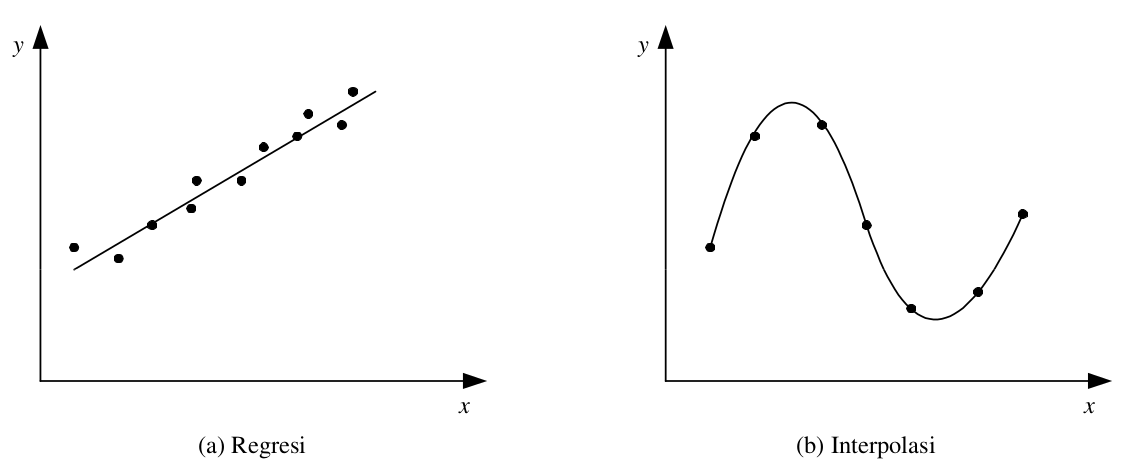
\includegraphics[width=\linewidth]{img/img02}
	\end{center}
\end{frame}

\begin{frame}
	\frametitle{Aplikasi Interpolasi Polinom}
	\begin{enumerate}
		\item Menghampiri fungsi rumit menjadi lebih sederhana
		\begin{itemize}
			\item Contoh: \[ f(x) = \frac{\ln(2x^{(1/2)}-4x^2)^3}{\sqrt{1+2x^5}} \]
			\item[] Hitung: $ f'(x) $ dan $\int f(x) dx$
			\item Perhitungan menjadi lebih mudah jika $ f(x) $ dihampiri dengan polinom $ p(x) $.
			\item Polinom $ p(x) $ diperoleh dengan menginterpolasi beberapa titik diskrit dari $ f(x) $
		\end{itemize}
		\item Menggambar kurva (jika hanya diketahui titik-titik diskrit saja)
	\end{enumerate}
\end{frame}

\section{Interpolasi Polinom}

\begin{frame}
	\frametitle{Interpolasi Polinom}
	\textbf{Persoalan}
	\begin{itemize}
		\item Diberikan $ n+1 $ buah titik berbeda, ($ x_0 $, $ y_0 $ ), ($ x_1 $, $ y_1 $ ), $\dots$, ($ x_n $ , $ y_n $ ).
		\item Tentukan polinom $ p_n(x) $ yang menginterpolasi (melewati) semua titik-titik tersebut sedemikian rupa sehingga
		\[ y_i = p_n(x_i)\qquad \text{ untuk } i = 0,1,2,\dots,n \]
		\item Nilai $ y_i $ dapat berasal dari fungsi $ f(x) $ sedemikian sehingga \[ y_i = f(x_i), \] atau, $ y_i $ berasal dari nilai empiris yang diperoleh melalui percobaan atau pengamatan.
	\end{itemize}
\end{frame}

\begin{frame}
	\begin{itemize}
		\item $ p_n(x) $ disebut fungsi hampiran terhadap $ f(x) $.
		\item Setelah polinom interpolasi $ p_n(x) $ ditemukan, $ p_n(x) $ dapat digunakan untuk menghitung perkiraan nilai $ y $ di $ x = a $, yaitu $ y = p_n(a) $.
		\item Bergantung pada letaknya, nilai $ x = a $ mungkin terletak di dalam rentang titik-titik data ($ x_0 < a < x_n $ ) atau di luar rentang titik-titik data ($ a < x_0 $ atau $ a > x_n $ ):
		\begin{enumerate}
			\item jika $ x_0 < a < x_n $ maka $ y_k = p(x_k) $ disebut \textbf{nilai interpolasi} (\textit{interpolated value})
			\item jika $ x_0 < x_k $ atau $ x_0 < x_n $ maka $ y_k = p(x_k) $ disebut nilai \textbf{ekstrapolasi} (\textit{extrapolated value}).
		\end{enumerate}
	\end{itemize}
\end{frame}

\begin{frame}
	\begin{center}
		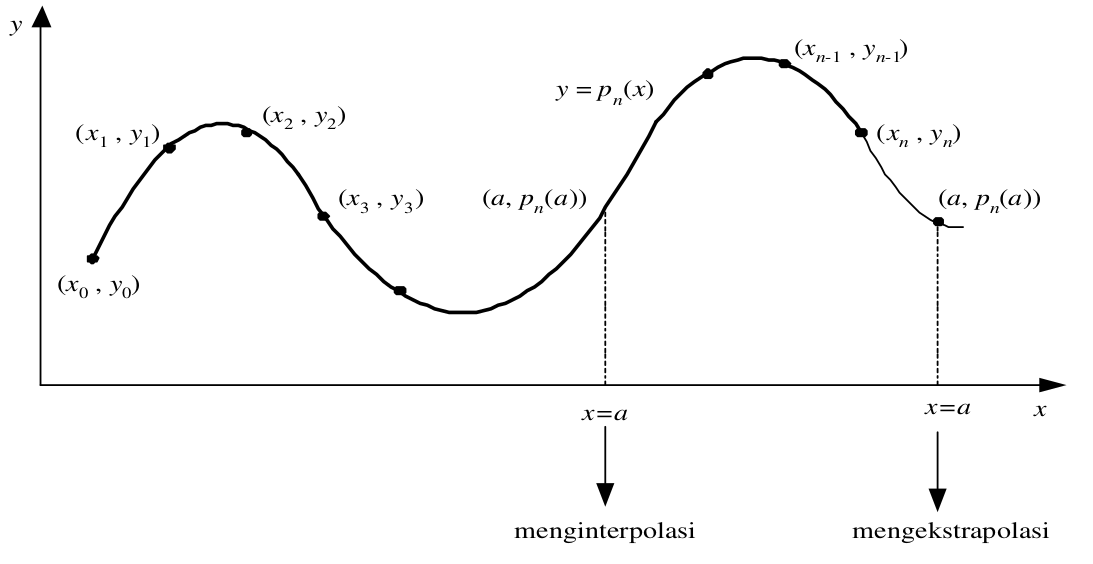
\includegraphics[width=0.7\linewidth]{img/img03}
	\end{center}
	\begin{itemize}
		\item Kita dapat menginterpolasi titik data dengan: polinom lanjar, polinom kuadratik, polinom kubik, atau polinom dari derajat yang lebih tinggi, bergantung pada jumlah titik data yang tersedia.
	\end{itemize}
\end{frame}

\subsection{Interpolasi Lanjar}

\begin{frame}
	\frametitle{Interpolasi Lanjar}
	\begin{itemize}
		\item Interpolasi lanjar adalah interpolasi dua buah titik dengan sebuah garis lurus.
		\item Misal diberikan dua buah titik, $ (x_0 , y_0) $ dan $ (x_1, y_1) $. Polinom yang menginterpolasi kedua titik itu adalah \[ p_1 (x) = a_0 + a_1 x \]
	\end{itemize}
	\begin{multicols}{2}
		\[ y_0 = a_0 + a_1 x_0;~y_1 = a_0 + a_1 x_1 \] menjadi
		\[ a_1 = \frac{y_1 - y_0}{x_1 - x_0};~a_0 = \frac{x_1 y_0 - x_0 y_1}{x_1 - x_0} \] sehingga
		\[ p_1(x) = \frac{x_1 y_0 - x_0 y_1}{x_1 - x_0} +  \frac{(y_1 - y_0)}{(x_1 - x_0)} x \]
		\columnbreak
		\begin{center}
			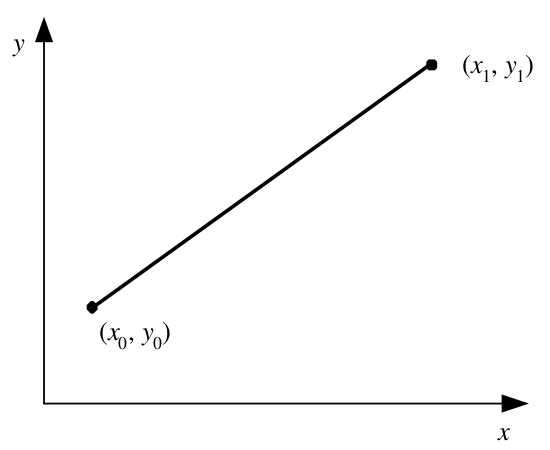
\includegraphics[width=0.8\linewidth]{img/img04}
		\end{center}
	\end{multicols}
\end{frame}

\begin{frame}
	Bila disederhanakan akan lebih lanjut:
	\begin{equation}\label{int.lanj}
		p_1(x) = y_0 + \frac{(y_1 - y_0)}{(x_1 - x_0)}(x-x_0)
	\end{equation}
\end{frame}

\begin{frame}
	\frametitle{Contoh 1}
	\begin{itemize}
		\item \textbf{Persoalan:} Perkirakan jumlah penduduk Amerika Serikat pada tahun 1968 berdasarkan data tabulasi berikut
		\begin{center}
			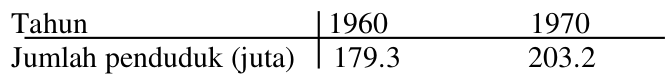
\includegraphics[width=0.8\linewidth]{img/img05}
		\end{center}
		\item \textbf{Penyelesaian:} Dengan menggunakan persamaan (\ref{int.lanj}) diperoleh
		\[ p_1(1968) = 179.3 + \frac{(203.2-179.3)(1968-1960)}{1970-1960} = 198.4 \]
		Jadi, taksiran jumlah penduduk AS pada tahun 1968 adalah 198.4 juta
	\end{itemize}
\end{frame}

\begin{frame}
	\frametitle{Contoh 2}
	\begin{itemize}
		\item \textbf{Persoalan:} Dari data $ \ln(9.0) = 2.1972 $, $ \ln(9.5) = 2.2513 $, tentukan $ \ln(9.2) $ dengan interpolasi lanjar sampai 5 angka bena. Bandingkan dengan nilai sejati $ ln(9.2) = 2.2192 $.
		\item \textbf{Penyelesaian:} Dengan menggunakan persamaan (\ref{int.lanj}), diperoleh
		\[ p_1(9.2) = 2.1972 + \frac{(2.1513-2.197)(9.2-9.0)}{9.5-90} = 2.2188 \]
		Galat = 2.2192 - 2.2188 = 0.0004. Di sini interpolasi lanjar tidak cukup untuk memperoleh ketelitian sampai 5 angka bena. Ia hanya benar sampai 3 angka bena
	\end{itemize}
\end{frame}

\subsection{Interpolasi Kuadratik}

\begin{frame}
	\frametitle{Interpolasi Kuadratik}
	\begin{itemize}
		\item Misal diberikan tiga buah titik data, $ (x_0, y_0) $, $ (x_1, y_1 ) $, dan $ (x_2, y_2) $.
		\item Polinom yang menginterpolasi ketiga buah titik itu adalah polinom kuadrat yang berbentuk:
		\begin{equation}\label{int.kuad}
			p_2(x) = a_0 + a_1x + a_2 x^2
		\end{equation}
		\begin{multicols}{2}
			\begin{center}
				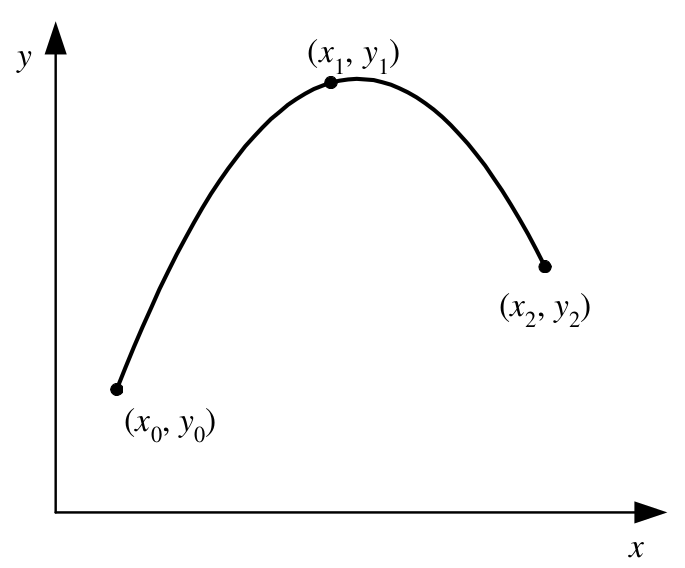
\includegraphics[width=\linewidth]{img/img06}
			\end{center}
			\item Bila digambar, kurva polinom kuadrat berbentuk parabola
		\end{multicols}
	\end{itemize}
\end{frame}

\begin{frame}{Interpolasi Kuadratik}
	Polinom $ p_2(x) $ ditentukan dengan cara berikut:
	\begin{enumerate}
		\item Sulihkan $ (x_i, y_i) $ ke dalam persamaan (\ref{int.kuad}), $ i = 0, 1, 2 $. Dari sini diperoleh tiga buah persamaan dengan tiga buah parameter yang tidak diketahui, yaitu $ a_0 $, $ a_1 $, dan $ a_2 $:
		\begin{align*}
			a_0 + a_1 x_0 + a_2 x_0^2 &= y_0\\
			a_0 + a_1 x_1 + a_2 x_1^2 &= y_1\\
			a_0 + a_1 x_2 + a_2 x_2^2 &= y_2
		\end{align*}
		\item hitung $ a_0 $, $ a_1 $, $ a_2 $ dari sistem persamaan tersebut dengan metode eliminasi Gauss.
	\end{enumerate}
\end{frame}

\begin{frame}
	\frametitle{Contoh 3}
	\begin{itemize}
		\item \textbf{Persoalan:} Diberikan titik $ \ln(8.0) = 2.0794 $, $ \ln(9.0) = 2.1972 $, dan $ \ln(9.5) = 2.2513 $. Tentukan nilai $ \ln(9.2) $ dengan interpolasi kuadratik.
		\item \textbf{Penyelesaian:} Sisten persamaan lanjar yang terbentuk adalah
		\begin{align*}
		a_0 + 8.0 a_1 + 64.00 a_2 &= 2.0794\\
		a_0 + 9.0 a_1 + 81.00 a_2 &= 2.1972\\
		a_0 + 9.5 a_1 + 90.25 a_2 &= 2.2513
		\end{align*}
		\item Penyelesaian sistem persamaan dengan metode eliminasi Gauss menghasilkan $ a_0 = 0.6762 $, $ a_1 = 0.2266 $, dan $ a_3 = -0.0064 $. Polinom
		kuadratnya adalah
		\[ p_2(x) = 0.6762 + 0.2266x - 0.0064x^2 \]
	\end{itemize}
\end{frame}

\begin{frame}{Contoh 3}
	\begin{itemize}
		\item sehingga \[ p_2(9.2) = 2.2192 \] yang sama dengan nilai sejatinya (5 angka bena).
	\end{itemize}
\end{frame}

\subsection{Interpolasi Kubik}

\begin{frame}
	\frametitle{Interpolasi Kubik}
	\begin{itemize}
		\item Misal diberikan empat buah titik data, $ (x_0, y_0) $, $ (x_1, y_1) $, $ (x_2, y_2) $,
		dan $ (x_3 , y_3) $.
		\item Polinom yang menginterpolasi keempat buah titik itu adalah polinom kubik yang berbentuk:
		\begin{equation}\label{int.kub}
			p_3(x) = a_0 + a_1x + a_2 x^2 + a_3 x^3
		\end{equation}
		\begin{center}
			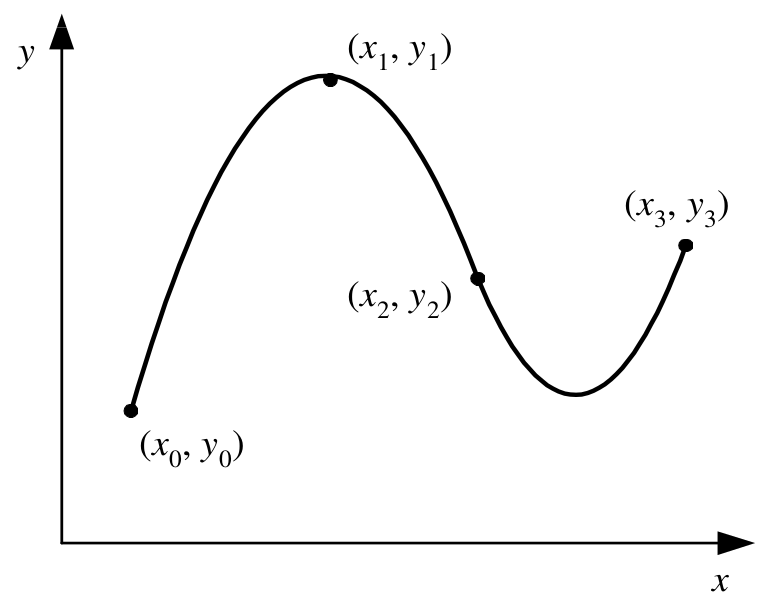
\includegraphics[width=0.4\linewidth]{img/img07}
		\end{center}
	\end{itemize}
\end{frame}

\begin{frame}{Interpolasi Kubik}
	Polinom $ p_3(x) $ ditentukan dengan cara berikut:
	\begin{enumerate}
		\item sulihkan $ (x_i, y_i) $ ke dalam persamaan \ref{int.kub} , $ i = 0, 1, 2, 3 $. Dari sini diperoleh empat buah persamaan dengan empat buah parameter yang tidak diketahui, yaitu $ a_0 $, $ a_1 $, $ a_2 $, dan $ a_3 $ :
		\begin{align*}
			a_0 + a_1 x_0 + a_2 x_0^2 + a_3 x_0^3 &= y_0 \\
			a_0 + a_1 x_1 + a_2 x_1^2 + a_3 x_1^3 &= y_1 \\
			a_0 + a_1 x_2 + a_2 x_2^2 + a_3 x_2^3 &= y_2 \\
			a_0 + a_1 x_3 + a_2 x_3^2 + a_3 x_3^3 &= y_3
		\end{align*}
		\item hitung $ a_0 $, $ a_1 $, $ a_2 $, dan $ a_3 $ dari sistem persamaan tersebut dengan metode eliminasi Gauss.
	\end{enumerate}
\end{frame}

\begin{frame}
	\begin{itemize}
		\item Dengan cara yang sama kita dapat membuat polinom interpolasi berderajat $ n $ untuk $ n $ yang lebih tinggi:
		\[ p_n(x) = a_0 + a_1 x + a_2 x^2 + \dots + a_n x^n \]
		asalkan tersedia $ (n+1) $ buah titik data.
		\item Dengan menyulihkan $ (x_i, y_i) $ ke dalam persamaan polinom di atas $ y = p_n(x) $ untuk $ i = 0, 1, 2, \dots, n $, akan diperoleh $ n $ buah sistem persamaan lanjar dalam $ a_0, a_1, a_2, \dots , a_n $,
		\begin{align*}
			a_0 + a_1 x_0 + a_2 x_0^2 + \dots + a_n x_0^3 &= y_0 \\
			a_0 + a_1 x_1 + a_2 x_1^2 + \dots + a_n x_1^3 &= y_1 \\
			&\vdots \\
			a_0 + a_1 x_n + a_2 x_n^2 + \dots + a_n x_n^3 &= y_n
		\end{align*}
		\item[] 
	\end{itemize}
\end{frame}

\begin{frame}
	\begin{itemize}
		\item Solusi sistem persamaan lanjar ini diperoleh dengan menggunakan metode eliminasi Gauss yang sudah anda pelajari.
		\item Secara umum, penentuan polinom interpolasi dengan cara yang diuraikan di atas kurang disukai,
		\item karena sistem persamaan lanjar yang diperoleh ada kemungkinan berkondisi buruk, terutama untuk derajat polinom yang semakin tinggi.
		\item Metode polinom interpolasi yang banyak digunakan dalam komputasi numerik adalah:
		\begin{enumerate}
			\item Polinom Lagrange
			\item Polinom Newton
			\item Polinom Newton-Gregory (kasus khusus dari polinom Newton)
		\end{enumerate}
	\end{itemize}
\end{frame}

\section{Polinom Lagrange}

\begin{frame}
	\frametitle{Polinom Lagrange}
	\begin{itemize}
		\item Tinjau kembali polinom lanjar:
		\[ p_1(x) = y_0 + \frac{(y_1 - y_0)}{(x_1 - x_0)}(x-x_0) \]
		\item Persamaan ini dapat diatur kembali sedemikian rupa sehingga menjadi
		\[ p_1(x) = y_0 + \frac{(x - x_1)}{(x_0 - x_1)} + y_1\frac{(x-x_0)}{(x_1-x_0)} \]
	\end{itemize}
\end{frame}

\begin{frame}{Polinom Lagrange}
	\begin{itemize}
		\item atau dapat dinyatakan dalam bentuk
		\[ p_1(x) = a_0 L_0 (x) + a_1 L_1 (x) \]
		\item yang dalam hal ini
		\[ a_0 = y_0,\quad L_0(x) = \frac{(x-x_1)}{(x_0-x_1)} \]
		dan
		\[ a_1 = y_1,\quad L_1(x) = \frac{(x-x_0)}{(x_1-x_0)} \]
	\end{itemize}
\end{frame}

\begin{frame}{Polinom Lagrange}
	\begin{itemize}
		\item Bentuk umum polinom Lagrange derajat $ \leq  n $ untuk $ (n + 1) $ titik berbeda adalah
		\begin{equation}\label{pol.lagr}
			p_n(x) = \sum_{i=0}^{n} a_i L_i(x) = a_0 L_0(x) + a_1 L_1(x) + \dots + a_n L_n(x)
		\end{equation}
		yang dalam hal ini
		\[ a_i = y_i,\quad i=0,1,2,\dots,n \]
		dan
		\begin{align*}
			L_i(x) &= \prod_{j=0;j\neq i}^{n} \frac{(x-x_j)}{(x_i-x_j)} \\
			&= \frac{(x-x_0)(x-x_1) \dots (x-x_{i-1})(x-x_{i+1})\dots (x-x_n)}{(x_i -x_0)(x_i-x_1) \dots (x_i-x_{i-1})(x_i-x_{i+1})\dots (x_i-x_n)}
		\end{align*}
	\end{itemize}
\end{frame}

\begin{frame}
	\frametitle{Contoh 4}
	\begin{itemize}
		\item \textbf{Persoalan:} Hampiri fungsi $ f(x) = \cos x $ dengan polinom interpolasi derajat tiga di dalam selang $ [0.0, 1.2] $. Gunakan empat titik, $ x_0 = 0.0 $, $ x_1 = 0.4 $, $ x_2 = 0.8 $, dan $ x_3 = 1.2 $. Perkirakan nilai $ p_3(0.5) $, dan bandingkan dengan nilai sejatinya.
		\item \textbf{Penyelesaian:}
		\begin{center}
			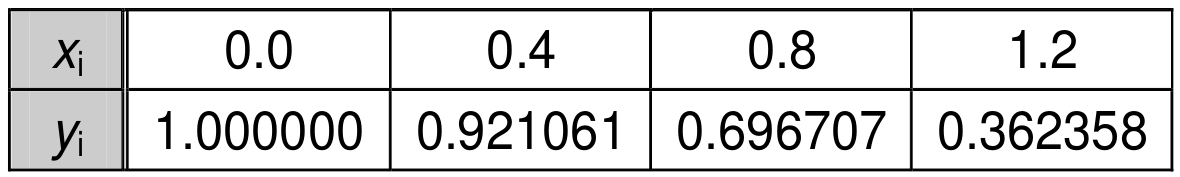
\includegraphics[width=0.7\linewidth]{img/img08}
		\end{center}
	\end{itemize}
\end{frame}

\begin{frame}{Contoh 4}
	\begin{itemize}
		\item Polinom Lagrange derajat 3 yang menginterpolasi keempat titik di tabel adalah
		\begin{align*}
			p_3 (x) &= a_0 L_0 (x) + a_1 L_1 (x) + a_2 L_2 (x) + a_3 L_3 (x) \\
			&= y_0 \frac{(x-x_1)(x-x_2)(x-x_3)}{(x_0-x_1)(x_0-x_2)(x_0-x_3)} \\
			&+ y_1 \frac{(x-x_1)(x-x_2)(x-x_3)}{(x_1-x_0)(x_1-x_2)(x_1-x_3)} \\
			&+ y_2 \frac{(x-x_1)(x-x_2)(x-x_3)}{(x_2-x_0)(x_2-x_1)(x_2-x_3)} \\
			&+ y_3 \frac{(x-x_1)(x-x_2)(x-x_3)}{(x_3-x_0)(x_3-x_1)(x_3-x_2)} \\
		\end{align*}
	\end{itemize}
\end{frame}

\begin{frame}{Contoh 4}
	\begin{itemize}
		\item[]
		\begin{align*}
		p_3 (x) &= 1.000000 \frac{(x-0.4)(x-0.8)(x-1.2)}{(0.0-0.4)(0.0-0.8)(0.0-1.2)} \\
		&+ 0.921061 \frac{(x - 0.0 )(x - 0.8)(x - 1.2)}{(0.4 - 0.0)( 0.4 - 0.8 )( 0.4 - 1.2 )} \\
		&+ 0.696707 \frac{(x - 0.0 )(x - 0.4)(x - 1.2)}{(0.8 - 0.0)( 0.8 - 0.4 )( 0.8 - 1.2 )} \\
		&+ 0.362358 \frac{(x - 0.0 )(x - 0.4)(x - 0.8)}{(1.2 - 0.0)( 1.2 - 0.4 )( 1.2 - 0.8 )} \\
		\end{align*}
	\end{itemize}
\end{frame}

\begin{frame}{Contoh 4}
	\begin{itemize}
		\item[]
		\begin{align*}
		p_3 (x) &= - 2.604167 ( x - 0.4 )( x - 0.8 )( x - 1.2 )
		&+ 7.195789 ( x - 0.0 )( x - 0.8 )( x - 1.2 ) \\
		&- 5.443021 ( x - 0.0 )( x - 0.4 )( x - 1.2 )\\
		&+ 0.943640 ( x - 0.0 )( x - 0.4 )( x - 0.8 )
		\end{align*}
	\end{itemize}
\end{frame}

\begin{frame}{Contoh 4}
	\begin{itemize}
		\item Untuk mengurangi galat akibat pembulatan, polinom $ p_3(x) $ ini tidak perlu disederhanakan lebih jauh. Kurva $ y = \cos(x) $ dan $ y = p_3(x) $ diperlihatkan pada Gambar berikut:
		\begin{center}
			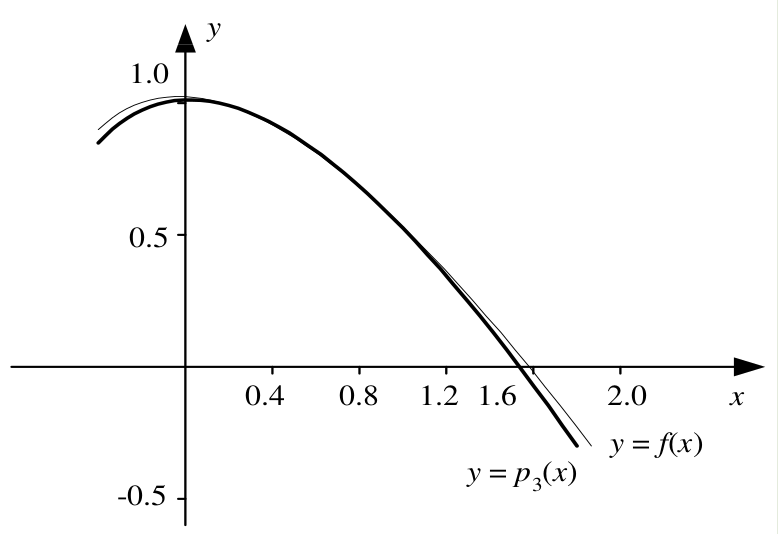
\includegraphics[width=0.7\linewidth]{img/img09}
		\end{center}
	\end{itemize}
\end{frame}

\begin{frame}{Contoh 4}
	\begin{itemize}
		\item Dengan menggunakan polinom interpolasi $ p_3 (x) $ itu kita dapat menaksir nilai fungsi di $ x = 0.5 $ sebagai berikut:
		\begin{align*}
			p_3(0.5) &= -2.604167(0.5 - 0.4)(0.5 - 0.8)(0.5 - 1.2) \\
			&+ 7.195789(0.5 - 0.0)(0.5 - 0.8)(0.5 - 1.2) \\
			&-5.443021(0.5 - 0.0)(0.5 - 0.4)(0.5 - 1.2) \\
			&+ 0.943640(0.5 - 0.0)(0.5 - 0.4)(0.5 - 0.8) \\
			&= 0.877221
		\end{align*}
		\item Sebagai perbandingan, nilai sejatinya adalah
		$ y = \cos(0.5) = 0.877583 $
	\end{itemize}
\end{frame}

\begin{frame}
	\frametitle{Contoh 5}
	\begin{itemize}
		\item \textbf{Persoalan:} Dari fungsi $ y = f(x) $, diberikan tiga buah titik data dalam bentuk tabel:
		\begin{center}
			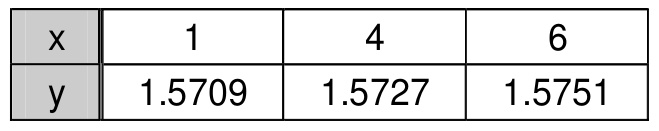
\includegraphics[width=0.7\linewidth]{img/img10}
		\end{center}
		Tentukan $ f(3.5) $ dengan polinom Lagrange derajat 2. Gunakan lima angka bena.
	\end{itemize}
\end{frame}

\begin{frame}{Contoh 5}
	\begin{itemize}
		\item \textbf{Penyelesaian:} Polinom derajat $ 2 \rightarrow n = 2 $ (perlu tiga buah titik)
		\[ p_2 (x) = L_0 (x) y_0 + L_1 (x) y_1 + L_2 (x) y_2 \]
	\end{itemize}
	\begin{align*}
		L_0(x) = \frac{( x - 4 )( x - 6 )}{( 1 - 4 )( 1 - 6 )} &\rightarrow L_0(3.5) = \frac{( 3 . 5 - 4 )( 3 . 5 - 6 )}{( 1 - 4 )( 1 - 6 )} = 0.083333 \\
		L_1(x) = \frac{( x - 1 )( x - 6 )}{( 4 - 1 )( 4 - 6 )} &\rightarrow L_1(3.5) = \frac{( 3 . 5 - 1 )( 3 . 5 - 6 )}{( 4 - 1 )( 4 - 6 )} = 1.0417 \\
		L_2(x) = \frac{( x - 1 )( x - 3 )}{( 6 - 1 )( 6 - 4 )} &\rightarrow L_2(3.5) = \frac{( 3 . 5 - 1 )( 3 . 5 - 4 )}{( 6 - 1 )( 6 - 4 )} = -0.12500 \\
	\end{align*}
		Jadi, $ p_2(3.5) = (0.083333)(1.5709) + (1.0417)(1.5727) + (-0.12500)(1.5751) = 1.5723 $
\end{frame}

\begin{frame}
	\frametitle{Komputasi Lagrange}
	\begin{itemize}
		\item Mari membuat algoritma dari Lagrange dan source code nya berbahasa Python
	\end{itemize}
\end{frame}

\section{Polinom Newton}

\begin{frame}
	\frametitle{Polinom Newton}
	Polinom Lagrange kurang disukai dalam praktek karena alasan berikut:
	\begin{enumerate}
		\item Jumlah komputasi yang dibutuhkan untuk satu kali interpolasi adalah besar. Interpolasi untuk nilai $ x $ yang lain memerlukan jumlah komputasi yang sama karena tidak ada bagian komputasi sebelumnya yang dapat digunakan.
		\item Bila jumlah titik data meningkat atau menurun, hasil komputasi sebelumnya tidak dapat digunakan. Hal ini disebakan oleh tidak adanya hubungan antara $ p_{n-1}(x) $ dan $ p_n(x) $ pada polinom Lagrange.
	\end{enumerate}
\end{frame}

\begin{frame}
	\begin{itemize}
		\item Alternatif: polinom Newton
		\item Polinom Newton dinyatakan dalam hubungan rekursif sebagai berikut:
		\begin{enumerate}
			\item rekurens: $ p_n(x) = p_{n-1}(x) + a_n(x - x_0)(x - x_1) \dots (x - x_{n-1} ) $
			\item basis: $ p_0(x) = a_0 $
		\end{enumerate}
		\item Jadi, tahapan pembentukan polinom Newton adalah sebagai berikut:
		\begin{align*}
			p_1(x) &= p_0(x) + a_1 (x - x_0) \\
			&= a_0 + a_1 (x - x_0)\\
			&\\
			p_2(x) &= p_1(x) + a_2 (x - x_0)(x - x_1) \\
			&= a_0 + a_1 (x - x_0) + a_2 (x - x_0)(x - x_1)
		\end{align*}
	\end{itemize}
\end{frame}

\begin{frame}
	\begin{itemize}
		\item[]
		\begin{align*}
			p_3(x) &= p_0(x) + a_3 (x - x_0)(x - x_1)(x - x_2) \\
			&= a_0 + a_1 (x - x_0) + a_2 (x - x_0)(x - x_1)\\
			&+ a_3 (x - x_0)(x - x_1)(x - x_2)\\
			&\\
			p_n(x) &= p_{n-1}(x) + a_n (x - x_0)\dots(x - x_{n-1})\\
			&= a_0 + a_1 (x - x_0) + a_2 (x - x_0)(x - x_1)\\
			&+ a_3 (x - x_0)(x - x_1)(x - x_2) + \dots \\
			&+  a_n (x - x_0)(x - x_1)\dots(x - x_{n-1})\\
		\end{align*}
	\end{itemize}
\end{frame}

\begin{frame}
	\begin{itemize}
		\item Nilai konstanta $ a_0 $, $ a_1 $, $ a_2 $, $\dots$, $ a_n $ merupakan nilai selisih-terbagi, (\textit{divided-diffrence}) dengan nilai masing-masing:
		\begin{align*}
		a_0 &= f(x_0) \\
		a_1 &= f(x_1,x_0) \\
		a_2 &= f(x_2,x_1,x_0) \\
		&\vdots\\
		a_n &= f(x_n, x_{n-1}, \dots, x_1, x_0) \\
		\end{align*}
	\end{itemize}
\end{frame}

\begin{frame}
	\begin{itemize}
		\item yang dalam hal ini
	\end{itemize}
	\begin{align*}
		f[x_i, x_j] &= \frac{f(x_i)-f(x_j)}{x_i - x_j} \\
		f[x_i, x_j, x_k] &= \frac{f[x_i, x_j] - f[x_j, x_k]}{x_i - x_k} \\
		\vdots&\\
		f[x_n, x_{n-1}, \dots, x_1, x_0] &= \frac{f[x_n, x_{n-1}, \dots, x_1] - f[x_{n-1},x_{n-2},\dots, x_0]}{x_n - x_0}
	\end{align*}
\end{frame}

\begin{frame}
	\begin{itemize}
		\item Dengan demikian polinom Newton dapat ditulis dalam hubungan rekursif sebagai
		\begin{enumerate}
			\item rekurens:
			\[\Scale[0.9]{ p_n(x) = p_{n-1}(x) + (x-x_0 ) (x-x_1) \dots (x-x_{n-1}) f[x_n , x_{n-1} , \dots, x_1 , x_0] }\]
			\item basis:
			\[ p_0(x) = f (x_0) \]
		\end{enumerate}
		\item atau dalam bentuk polinom yang lengkap sebagai berikut:
		\begin{align*}
			p_n(x) &= f_(x_0) + (x-x_0)f[x_1, x_0] + (x-x_0)(x-x_1) f[x_2, x_1, x_0] \\
			&+ (x - x_0) (x - x_1) \dots (x - x_{n-1}) f[x_n, x_{n-1} , \dots, x_1, x_0]
		\end{align*}
	\end{itemize}
\end{frame}

\begin{frame}
	\begin{itemize}
		\item Nilai selisih terbagi ini dapat dihitung dengan menggunakan tabel yang disebut tabel selisih-terbagi,
		\item misalnya tabel selisih-terbagi untuk empat buah titik ($ n = 3 $) berikut:
	\end{itemize}
	\begin{center}
		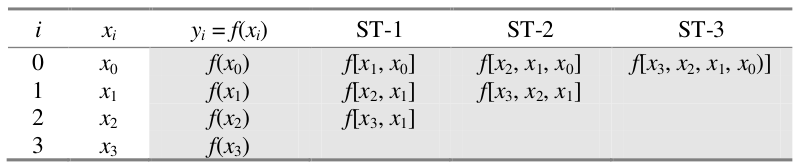
\includegraphics[width=\linewidth]{img/img11}
	\end{center}
	Keterangan: ST = Selisih-Terbagi
\end{frame}

\begin{frame}
	\frametitle{Komputasi Polinom Newton}
	\begin{itemize}
		\item Mari membuat algoritma dari polinom Newton dan source code nya berbahasa Python
	\end{itemize}
\end{frame}

\begin{frame}
	\frametitle{Contoh 6}
	\begin{itemize}
		\item \textbf{Persoalan:} Hitunglah $ f(9.2) $ dari nilai-nilai $ (x, y) $ yang diberikan pada tabel di bawah ini dengan polinom Newton derajat 3.
		\begin{center}
			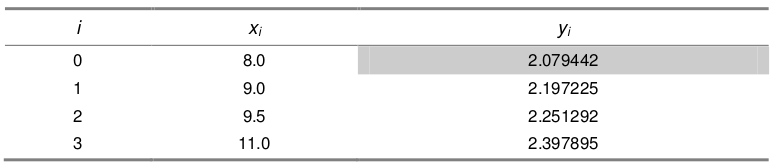
\includegraphics[width=\linewidth]{img/img12}
		\end{center}
	\end{itemize}
\end{frame}

\begin{frame}{Contoh 6}
	\begin{itemize}
		\item \textbf{Penyelesaian:} Tabel selisih-terbagi:
		\begin{center}
			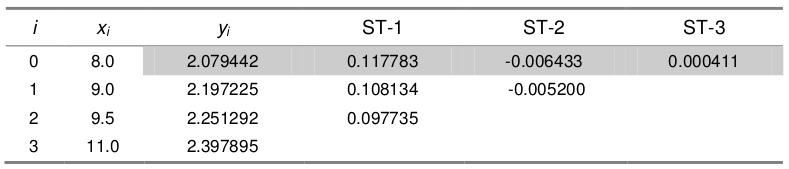
\includegraphics[width=\linewidth]{img/img13}
		\end{center}
		\item Contoh cara menghitung nilai selisih-terbagai pada tabel adalah:
		\begin{align*}
			f(x_2, x_1) &= \frac{f(x_2) - f(x_1)}{x_2 - x_1} = \frac{2.251292 - 2.197225}{9.5 - 9.0} = 0.108134 \\
			f(x_2, x_1, x_0) &= \frac{f[x_2,x_1] - f[x_1,x_0]}{x_2 - x_0}\\
			&= \frac{0.108134 - 0.117783}{9.5 - 8.0} = -0.006433 \\
			&\text{dan seterusnya}
		\end{align*}
	\end{itemize}
\end{frame}

\begin{frame}{Contoh 6}
	\begin{itemize}
		\item Polinom Newton-nya (dengan $ x_0 = 8.0 $ sebagai titik data pertama) adalah:
		\begin{align*}
			f(x) &\approx p_3(x) = 2.079442 + 0.117783(x - 8.0)\\
			&- 0.006433(x - 8.0)x - 9.0) \\
			&+ 0.000411(x - 8.0)(x - 9.0)(x - 9.5)
		\end{align*}
		\item Taksiran nilai fungsi pada $ x = 9.2 $ adalah
		\begin{align*}
			f(9.2) \approx p_3(9.2) &= 2.079442 + 0.141340 - 0.001544 - 0.000030 \\
			&= 2.219208
		\end{align*}
	\end{itemize}
\end{frame}

\begin{frame}
	\frametitle{Contoh 7}
	\begin{itemize}
		\item \textbf{Persoalan:} Bentuklah polinom Newton derajat satu, dua, tiga, dan empat yang menghampiri fungsi $ f(x) = \cos(x) $ di dalam selang $ [0.0 , 4.0] $ dan jarak antar titik adalah $ 1.0 $. Lalu, taksirlah nilai fungsi di $ x = 2.5 $ dengan polinom Newton derajat tiga
	\end{itemize}
\end{frame}

\begin{frame}{Contoh 7}
	\begin{itemize}
		\item \textbf{Penyelesaian:} Dengan jarak antar titik 1.0, maka titik yang digunakan adalah pada $ x_0 = 0.0 $, $ x_1 = 1.0 $, $ x_2 = 3.0 $, $ x_3 = 4.0 $. Tabel selisih terbaginya adalah:
		\begin{center}
			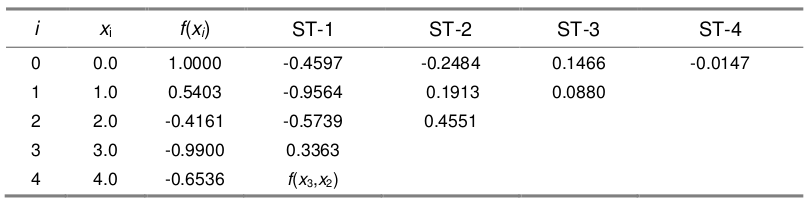
\includegraphics[width=\linewidth]{img/img14}
		\end{center}
	\end{itemize}
\end{frame}

\begin{frame}{Contoh 7}
	Maka, polinom Newton derajat 1, 2, dan 3 dengan $ x_0 = 0.0 $ sebagai titik data pertama adalah
	\begin{align*}
		\cos(x) \approx p_1(x) &= 1.0000 - 0.4597(x - 0.0) \\
		\cos(x) \approx p_2(x) &= 1.0000 - 0.4597(x - 0.0) - 0.2484(x - 0.0)(x - 1.0) \\
		\cos(x) \approx p_3(x) &= 1.0000 - 0.4597(x - 0.0) - 0.2484(x - 0.0)(x - 1.0) \\
		&+ 0.1466(x - 0.0)(x - 1.0)(x - 2.0) \\
		\cos(x) \approx p_4(x) &= 1.0000 - 0.4597(x - 0.0) - 0.2484(x - 0.0)(x - 1.0) \\
		&+ 0.1466(x - 0.0)(x - 1.0)(x - 2.0) \\
		&-0.0147(x - 0.0)(x - 1.0)(x - 2.0)(x - 3.0)
	\end{align*}
\end{frame}

\begin{frame}{Contoh 7}
	\begin{center}
		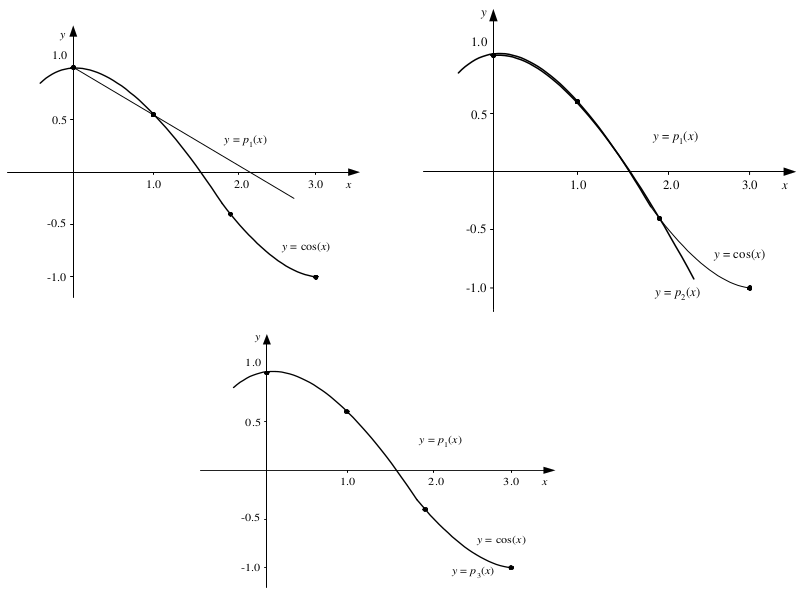
\includegraphics[width=0.8\linewidth]{img/img15}
	\end{center}
\end{frame}

\begin{frame}{Contoh 7}
	\begin{itemize}
		\item Taksiran nilai fungsi di $ x = 2.5 $ dengan polinom derajat tiga adalah
		\begin{align*}
			\cos(2.5) \approx p_3(2.5) &= 1.0000 - 0.4597(2.5 - 0.0)\\
			&- 0.2484(2.5 - 0.0)(2.5 - 1.0)\\
			&+ 0.1466(2.5 - 0.0)(2.5 - 1.0)(2.5 - 2.0) \\
			&\approx -0.8056
		\end{align*}
		\item Nilai sejati $ f(2.5) $ adalah
		\[ f(2.5) = \cos(2.5) = -0.8011 \]
		\item sehingga solusi hampiran mengandung galat sejati sebesar
		\[ \varepsilon = -0.8011 - (-0.8056) = -0.0045 \]
	\end{itemize}
\end{frame}

\begin{frame}
	\frametitle{Kelebihan Polinom Newton}
	\begin{itemize}
		\item Karena polinom Newton dibentuk dengan menambahkan satu suku tunggal dengan polinom derajat yang lebih rendah, maka ini memudahkan perhitungan polinom derajat yang lebih tinggi dalam program yang sama. Karena alasan itu, polinom Newton sering digunakan khususnya pada kasus yang derajat polinomnya tidak diketahui terlebih dahulu.
		\item Penambahan suku-suku polinom secara beruntun dapat dijadikan kriteria untuk menentukan tercapainya titik berhenti, yaitu apakah penambahan suku-suku yang lebih tinggi tidak lagi secara berarti memperbaiki nilai interpolasi, atau malahan menjadi lebih buruk.
		\item Tabel selisih terbagi dapat dipakai berulang-ulang untuk memperkirakan nilai fungsi pada nilai $ x $ yang berlainan.
	\end{itemize}
\end{frame}

\begin{frame}
	\frametitle{Galat Interpolasi Polinom}
	\begin{align*}
		E(x) &= f(x) - p_n(x)\\
		&= (x - x_0) (x - x_1) ... (x - x_n) \frac{f^{(n+1)}(c)}{(n+1)!}
	\end{align*}
	\begin{itemize}
		\item Dari rumus di atas, galat polinom interpolasi, selain bergantung pada nilai $ x $ yang diinterpolasi, juga bergantung pada turunan fungsi semula.
		\item Tinjau $ Q_{n+1} $ pada rumus $ E(x) $
		\[ Q_{n+1}(x) = (x - x_0)(x - x_1) \dots (x - x_n) \]
	\end{itemize}
\end{frame}

\begin{frame}{Galat Interpolasi Polinom}
	\begin{itemize}
		\item Misalkan $ x_0, x_1 , \dots, x_n $ berjarak sama. Grafik fungsi $ Q $ untuk enam titik yang berjarak sama ditunjukkan pada Gambar:
		\begin{center}
			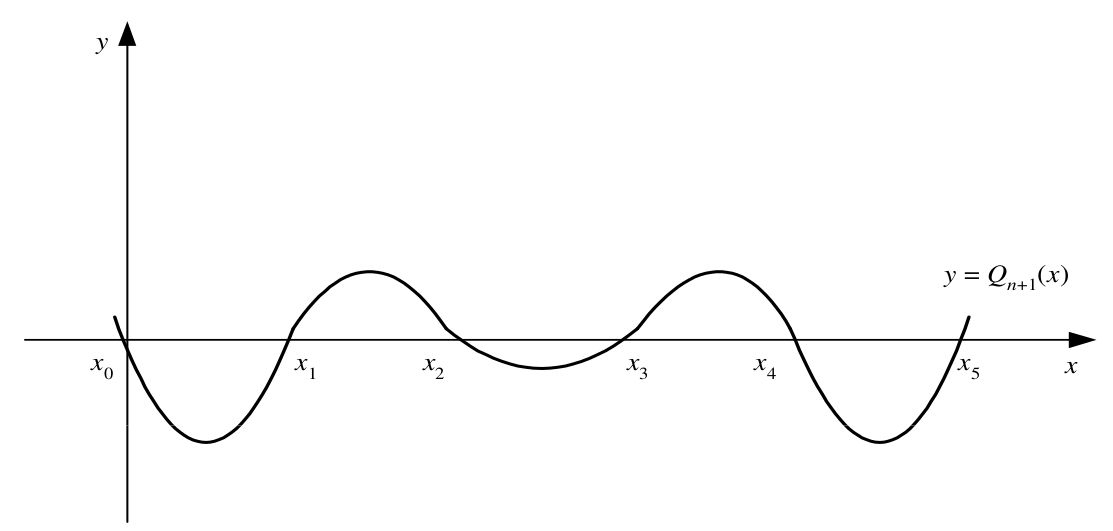
\includegraphics[width=0.8\linewidth]{img/img16}
		\end{center}
	\end{itemize}
\end{frame}

\begin{frame}{Galat Interpolasi Polinom}
	\begin{itemize}
		\item Berdasarkan $ Q_6(x) $ yang berosilasi pada Gambar di atas terlihat bahwa:
		\begin{enumerate}
			\item di titik-titik data $ x_i $ , nilai $ Q_6(x_i) = 0 $, sehingga galat interpolasi $ E(x_i)=0 $
			\item di titik tengah selang, nilai $ Q_6(x) $ minimum, sehingga $ E(x) $ juga minimum
			\item di titik-titik sekitar ujung selang, $ Q_6(x) $ besar, sehingga $ E(x) $ juga besar
			\item bila ukuran selang $ [x_0 , x_6] $ semakin besar, amplitudo osilasi meningkat dengan cepat.
		\end{enumerate}
	\end{itemize}
\end{frame}

\begin{frame}{Galat Interpolasi Polinom}
	\begin{itemize}
		\item \textbf{Kesimpulan:} Galat interpolasi minimum terjadi untuk nilai $ x $ di pertengahan selang.
		\begin{center}
			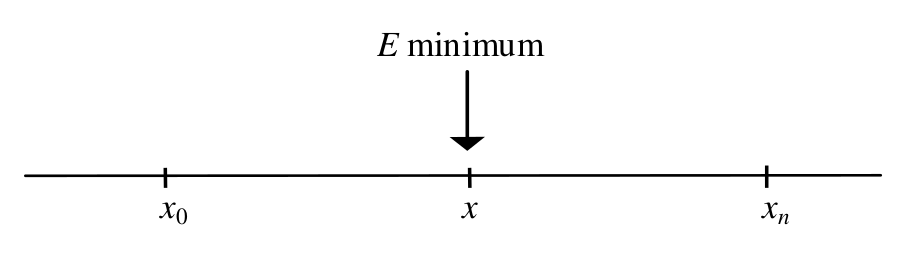
\includegraphics[width=0.8\linewidth]{img/img17}
		\end{center}
		\item \textbf{Ingatlah kalimat ini:}
		\item[] Untuk mendapatkan galat interpolasi yang minimum,
		pilihlah selang $ [x_0, x_n] $ sedemikian sehingga $ x $ terletak di tengah selang tersebut.
	\end{itemize}
\end{frame}

\begin{frame}{Galat Interpolasi Polinom}
	\begin{itemize}
		\item Misalkan kepada kita diberikan titik-titik data seperti ini:
		\begin{center}
			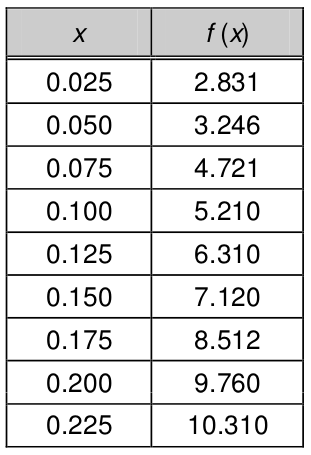
\includegraphics[width=0.3\linewidth]{img/img18}
		\end{center}
	\end{itemize}
\end{frame}

\begin{frame}{Galat Interpolasi Polinom}
	\begin{itemize}
		\item Bila anda diminta menghitung $ f(0.160) $, maka selang yang digunakan agar galat interpolasi $ f(0.160) $ kecil adalah
		\begin{itemize}
			\item[] $ [0.150, 0.175] \rightarrow $ untuk polinom derajat satu, atau
			\item[] $ [0.125, 0.200] \rightarrow $ untuk polinom derajat tiga, atau
			\item[] $ [0.100, 0.225] \rightarrow $ untuk polinom derajat lima
		\end{itemize}
	\end{itemize}
\end{frame}

\section{Polinom Newton-Gregory}

\begin{frame}
	\frametitle{Polinom Newton-Gregory}
	\begin{itemize}
		\item Polinom Newton-Gregory merupakan kasus khusus dari polinom Newton untuk titik-titik yang berjarak sama.
		\item Untuk titik-titik yang berjarak sama, rumus polinom Newton menjadi lebih sederhana. Selain itu, tabel selisih-terbaginya pun lebih mudah dibentuk. Di sini kita menamakan tabel tersebut sebagai \textbf{tabel selisih} saja.
		\item Ada dua macam tabel selisih, yaitu tabel selisih maju (\textit{forward difference}) dan tabel selisih mundur (\textit{backward difference}).
		\item Karena itu, ada dua macam polinom Newton-Gregory, yaitu polinom \textbf{Newton-Gregory maju} dan polinom \textbf{Newton-Gregory mundur}.
	\end{itemize}
\end{frame}

\subsection{Polinom Newton-Gregory Maju}

\begin{frame}
	\frametitle{Polinom Newton-Gregory Maju}
	\begin{itemize}
		\item Misalkan tabel selisih maju yang dibentuk dari lima buah titik:
		\begin{center}
			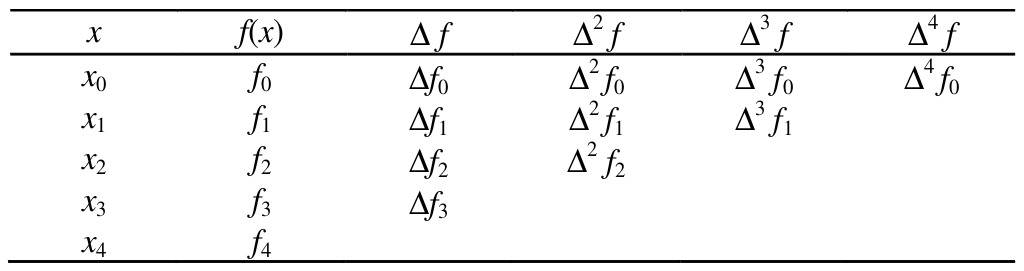
\includegraphics[width=\linewidth]{img/img19}
		\end{center}
		\item Bentuk umum:
		\[ \Delta^{n+1}f_p = \Delta^{n}f_{p+1} - \Delta^{n}f_p,\quad n=0,1,2,\dots \]
	\end{itemize}
\end{frame}

\begin{frame}
	\frametitle{Penurunan Rumus Polinom Newton-Gregory Maju}
	\begin{align*}
		f[x_1,x_0] &= \frac{f(x_1) - f(x_0)}{x_1-x_0} = \frac{\Delta f(x_0)}{h} = \frac{\Delta f_0}{1!h} \\
		f[x_1, x_2, x_0] &= \frac{f[x_2,x_1] - f[x_1,x_0]}{x_2-x_0} = \frac{\frac{f(x_2) - f(x_1)}{x_2-x_1} - \frac{f(x_1) - f(x_0)}{x_1-x_0}}{x_2-x_0} \\
		&= \frac{\frac{\Delta f_1 - \Delta f_0}{h}}{2h} = \frac{\Delta^2 f_0}{h}\frac{1}{2h} = \frac{\Delta^2f_0}{2!h^2}
	\end{align*}
	\begin{itemize}
		\item Bentuk umum:
		\[ f[x_n,\dots,x_1,x_0] = \frac{\Delta^n f(x_0)}{n!h^n} \]
	\end{itemize}
\end{frame}

\begin{frame}{Penurunan Rumus Polinom Newton-Gregory Maju}
	\begin{itemize}
		\item Dengan demikian polinom Newton untuk data berjarak sama dapat ditulis sebagai:
	\end{itemize}
	\begin{align*}
		p_n(x) &= f(x_0) + (x - x_0) f[x_1, x_0] + (x - x_0 )(x - x_1)f(x_2, x_1, x_0) \\
		&+ \dots + (x - x_0)(x-x_1)\dots(x-x_{n-1})f[x_n, x_{n-1} , \dots, x_1, x_0] \\
		&= f_0 + (x - x_0) \frac{\Delta f_0}{1!h} + (x - x_0)(x - x_1)\frac{\Delta^2 f_0}{2!h^2} \\
		& + \dots + (x - x_0)(x - x_1)\dots(x - x_{n-1})\frac{\Delta^n f_0}{n!h^n}
	\end{align*}
	\begin{itemize}
		\item Persamaan ini dinamakan polinom Newton-Gregory maju.
	\end{itemize}
\end{frame}

\begin{frame}{Penurunan Rumus Polinom Newton-Gregory Maju}
	\begin{itemize}
		\item Persamaan di atas dapat juga ditulis sebagai relasi rekursif:
		\[ p_n(x) = p_{n-1}(x) + (x-x_0)(x-x_1)\dots(x-x_{n-1})\frac{\Delta^nf_0}{n!h^n}\]
		\item Jika titik-titik berjarak sama dinyatakan sebagai
		\[ x_i = x_0 + ih,\quad i = 0,1,2,\dots,n \]
		\item dan nilai $ x $ yang diinterpolasikan adalah
		\[ x = x_0 + sh,\quad s \in R \]
	\end{itemize}
\end{frame}

\begin{frame}{Penurunan Rumus Polinom Newton-Gregory Maju}
	\begin{itemize}
		\item maka, persamaan di atas dapat juga ditulis dalam parameter $ s $ sebagai
		\begin{align*}
			p_n(x) &= f_0 + \frac{sh}{1!h}\Delta f_0 + \frac{s(s-1)h^2}{2!h^2}\Delta^2 f_0 + \dots + \\
			& \frac{s(s-1)(s-2) \dots (s-n+1)h^n}{n!h^n}\Delta^n f_0
		\end{align*}
		\item yang menghasilkan
		\begin{align*}
			p_n(x) &= f_0 + \frac{s}{1!}\Delta f_0 + \frac{s(s-1)}{2!}\Delta^2 f_0 + \dots + \\
			& \frac{s(s-1)(s-2) \dots (s-n+1)}{n!}\Delta^n f_0
		\end{align*}
	\end{itemize}
\end{frame}

\begin{frame}{Penurunan Rumus Polinom Newton-Gregory Maju}
	\begin{itemize}
		\item atau dalam bentuk relasi rekursif,
		\begin{enumerate}
			\item rekurens:
			\[ p_n(x) = p_{n-1}(x) + \frac{s(s-1)(s-2) \dots (s-n+1)}{n!}\Delta^n f_0 \]
			\item basis:
			\[ p_0(x) = f(x_0) \]
		\end{enumerate}
	\end{itemize}
\end{frame}

\begin{frame}
	\frametitle{Contoh 8}
	\begin{itemize}
		\item \textbf{Persoalan:} Bentuklah tabel selisih untuk fungsi $ f(x) = 1/(x+1) $ di dalam selang $ [0.000, 0.625] $ dan $ h = 0.125 $. Hitung $ f(0.300) $ dengan polinom Newton-Gregory maju derajat 3.
	\end{itemize}
\end{frame}

\begin{frame}{Contoh 8}
	\begin{itemize}
		\item \textbf{Penyelesaian:} Tabel selisih maju:
	\end{itemize}
	\begin{center}
		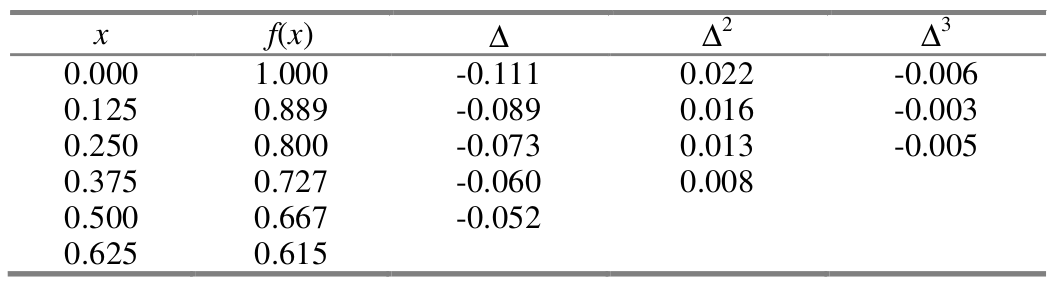
\includegraphics[width=\linewidth]{img/img20}
	\end{center}
\end{frame}

\begin{frame}{Contoh 8}
	\begin{itemize}
		\item Untuk memperkirakan f(0.300) dengan polinom Newton-Gregory maju derajat tiga, dibutuhkan 4 buah titik. Ingatlah kembali bahwa galat interpolasi akan minimum jika x terletak di sekitar pertengahan selang. Karena itu, titik-titik yang diambil adalah
		\[ x_0 = 0.125,~ x_1 = 0.250,~ x_2 = 0.375,~ x_3 = 0.500 \]
		\item karena $ x = 0.300 $ terletak di sekitar pertengahan selang $ [0.125, 0.500] $.
	\end{itemize}
\end{frame}

\begin{frame}{Contoh 8}
	\begin{itemize}
		\item Diketahui $ h = 0.125 $ dan
		\[ x = x_0 + sh \rightarrow s = \frac{x - x_0}{h} = \frac{0.310 - 0.125}{0.125} = 1.4 \]
		\item Nilai $ f(0.300) $ dihitung dengan polinom Newton-Gregory maju derajat tiga:
		\begin{align*}
			p_3(x) &\approx f_0 + \frac{s}{1!} \Delta f_0 + \frac{s(s-1)}{2!}\Delta^2 f_0 + \frac{s(s-1)(s-2)}{3!}\Delta^3 f_0 \\
			& \approx 0.889 + (1.4)(-0.089) + \frac{(1.4)(0.4)}{2}(0.016) + \frac{(1.4)(0.4)(-0.6)}{6}(-0.003) \\
			&\approx 0.889 - 0.1246 + 0.0045 \\
			&\approx 0.769
		\end{align*}
	\end{itemize}
\end{frame}

\begin{frame}{Contoh 8}
	\begin{itemize}
		\item Sebagai perbandingan, nilai sejati $ f(0.300) $ adalah $ f(0.300) = 1/(0.300+1) = 0.769 $
	\end{itemize}
\end{frame}

\begin{frame}
	\frametitle{Manfaat Tabel Selisih Maju}
	\begin{itemize}
		\item Misalkan kita membentuk tabel selisih untuk fungsi $ f(x) = x $, $ f(x) = x^2 $, dan $ f(x) = x^3 $ pada titik-titik x yang berjarak sama, yaitu $ x_i = x_0 + ih $, $ i = 0, 1, 2, 3, \dots $
		\item Tabel 1
		\begin{center}
			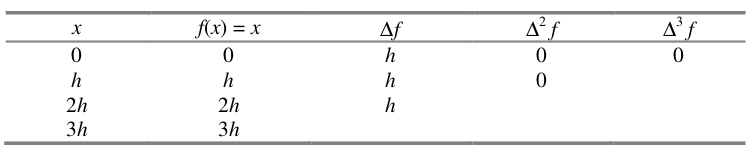
\includegraphics[width=0.7\linewidth]{img/img21}
		\end{center}
		\item Tabel 2
		\begin{center}
			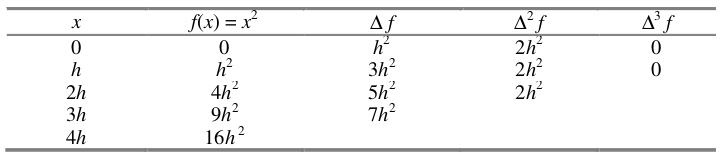
\includegraphics[width=0.7\linewidth]{img/img22}
		\end{center}
	\end{itemize}
\end{frame}

\begin{frame}{Manfaat Tabel Selisih Maju}
	\begin{itemize}
		\item Tabel 3
		\begin{center}
			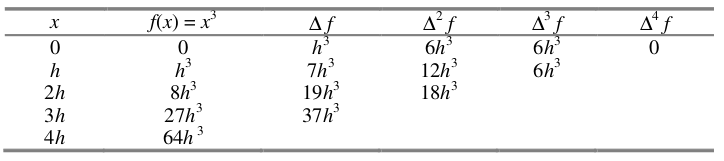
\includegraphics[width=0.7\linewidth]{img/img23}
		\end{center}
		\item Pada ketiga tabel itu dapat disimpulkan bahwa untuk $ f(x) = ax^n $, yang dalam hal ini $ a = 1 $ dan $ n = 1, 2, 3 $, diperoleh
		\[ \Delta^n f(x) = a n! h^n \] dan \[ \Delta^{n+1} f(x) = 0 \]
	\end{itemize}
\end{frame}

\begin{frame}{Manfaat Tabel Selisih Maju}
	\begin{itemize}
		\item Bila di dalam tabel selisih ditemukan $ \Delta^k $ bernilai (hampir) konstan ($\neq 0$) maka polinom yang tepat menginterpolasi titik- titik itu adalah polinom berderajat $ k $.
		\item Pada contoh tabel 3 di atas: $ \Delta^3 $ konstan, jadi titik-titiknya tepat diinterpolasi dengan polinom derajat tiga (sama dengan fungsi aslinya, $ f(x) = x^3 $ )
		\item Bagaimanakah jika tidak terdapat $\Delta$ yang bernilai tetap ? Misalnya diberikan tabel selisih di bawah ini:
	\end{itemize}
\end{frame}

\begin{frame}{Manfaat Tabel Selisih Maju}
	\begin{center}
		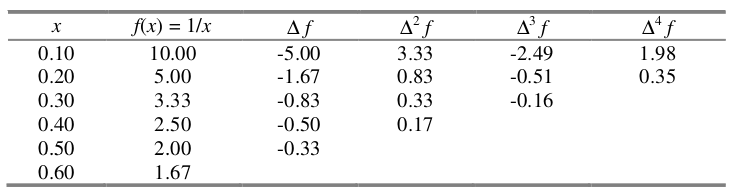
\includegraphics[width=0.7\linewidth]{img/img24}
	\end{center}
	\begin{itemize}
		\item Pada tabel selisih di atas, tidak ada $\Delta^k$ yang mendekati nilai tetap. Jadi $ f(x) = 1/x $ tidak tepat dihampiri dengan polinom derajat 1, 2, 3, atau 4 di dalam selang $ [0.10, 0.60] $.
	\end{itemize}
\end{frame}

\begin{frame}{Manfaat Tabel Selisih Maju}
	\begin{itemize}
		\item Tetapi jika selang datanya diperkecil dengan pengambilan $ h $ yang lebih kecil dan digunakan empat angka bena sebagai berikut:
		\begin{center}
			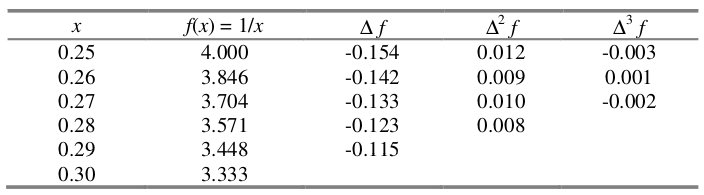
\includegraphics[width=0.7\linewidth]{img/img25}
		\end{center}
		\item maka dari tabel ini ditemukan $\Delta^2$ mendekati nilai tetap yaitu sekitar 0.010.
		\item Karena itu $ f(x) = 1/x $ dapat dihampiri sebanyak empat angka bena dengan polinom kuadratik di dalam selang $ [0.25, 0.30] $.
	\end{itemize}
\end{frame}

\begin{frame}
	\frametitle{Kesimpulan}
	\begin{itemize}
		\item Tabel selisih bermanfaat untuk menentukan
		\begin{enumerate}
			\item Derajat polinom interpolasi
			\item Selang data
			\item Ketelitian yang diinginkan.
		\end{enumerate}
	\end{itemize}
\end{frame}

\subsection{Polinom Interpolasi Newton-Gregory Mundur}

\begin{frame}
	\frametitle{Polinom Interpolasi Newton-Gregory Mundur}
	\begin{itemize}
		\item Polinom Newton-Gregory mundur (\textit{Newton-Gregory backward}) dibentuk dari tabel selisih mundur.
		\item Polinom ini sering digunakan pada perhitungan nilai turunan (\textit{derivative}) secara numerik. Titik-titik yang digunakan berjarak sama, yaitu
		\[ x_0,~x_{-1},~\dots,~x_{-n} \] yang dalam hal ini \[ x_i = x_0 + ih,\quad i = 0, -1, -2,\dots,-n \] dan nilai $ x $ yang diinterpolasikan adalah \[ x = x_0 + sh,~ s \in R \]
	\end{itemize}
\end{frame}

\begin{frame}{Polinom Interpolasi Newton-Gregory Mundur}
	\begin{itemize}
		\item Sebagai contoh, tabel selisih mundur untuk 4 titik diperlihatkan oleh tabel berikut
		\begin{center}
			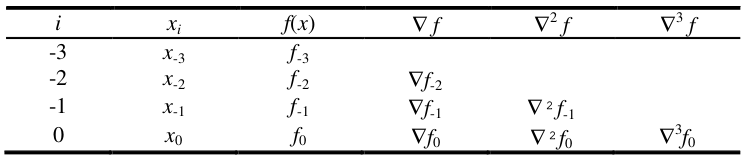
\includegraphics[width=\linewidth]{img/img26}
		\end{center}
	\end{itemize}
\end{frame}

\begin{frame}{Polinom Interpolasi Newton-Gregory Mundur}
	\begin{itemize}
		\item Polinom Newton-Gregory mundur yang menginterpolasi $ (n+1) $ titik data adalah
		\begin{align*}
			f(x) \approx p_n(x) &= \sum_{k=0}^{n} \left(\begin{matrix}
			s+k-1 \\ s
			\end{matrix}\right) \triangledown ^k f_0 \\
			&= f_0 + \frac{s\triangledown f_0}{1!} + \frac{s(s+1)\triangledown^2 f_0}{2!} \\
			&+ \dots + \frac{s(s+1)(s+2)\dots(s+n-1)\triangledown^n f_0}{n!}
		\end{align*}
	\end{itemize}
\end{frame}

\begin{frame}
	\frametitle{Contoh 9}
	\begin{itemize}
		\item \textbf{Persoalan:} Diberikan 4 buah titik data dalam tabel berikut. Hitunglah $ f(1.72) $ dengan
		\begin{enumerate}
			\item polinom Newton-Gregory maju derajat 3
			\item polinom Newton-Gregory mundur derajat 3
		\end{enumerate}
		Misalkan jumlah angka bena yang digunakan adalah 7 digit.
	\end{itemize}
\end{frame}

\begin{frame}{Contoh 9}
	\begin{itemize}
		\item \textbf{Penyelesaian:} 
		\begin{enumerate}
			\item Polinom Newton-Gregory maju derajat 3
			\begin{center}
				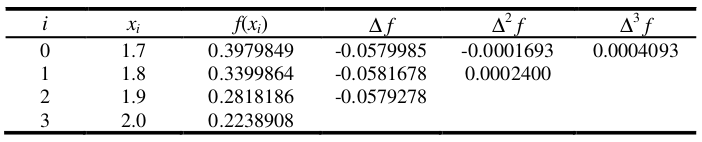
\includegraphics[width=\linewidth]{img/img27}
			\end{center}
			\[ s = (x - x_0)/h = (1.72 - 1.70)/0.1 = 0.2 \]
		\end{enumerate}
	\end{itemize}
\end{frame}

\begin{frame}{Contoh 9}
	\begin{itemize}
		\item[]
		\begin{enumerate}
			\item[] Perkiraan nilai $ f(1.72) $ adalah
			\begin{align*}
			f(1.72) &\approx p_3(1.72) = 0.3979849 + 0.2(-0.0579985) \\
			&+ \frac{0.2(-0.8)}{2}(-0.0001693) \\
			&+ \frac{0.2(-0.8)(-0.8)}{6}(0.0004093) \\
			&= 0.3979849 - 0.0115997 + 0.0000135 + 0.0000196 \\
			&= 0.3864183
			\end{align*}
		\end{enumerate}
		\item[] (nilai sejati $ f(1.72) = 0.3864185 $, jadi $ p_3(1.72) $ tepat sampai 6 angka bena)
	\end{itemize}
\end{frame}

\begin{frame}{Contoh 9}
	\begin{itemize}
		\item[]
		\begin{enumerate}
			\setcounter{enumi}{1}
			\item Polinom Newton-Gregory mundur derajat 3
			\begin{center}
				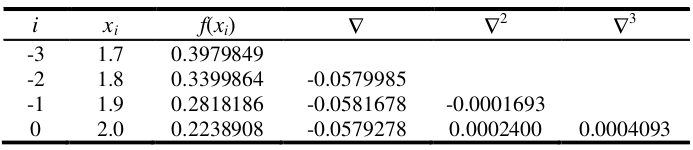
\includegraphics[width=\linewidth]{img/img28}
			\end{center}
			Tabel di atas memperlihatkan bahwa tabel selisih mundur sama dengan tabel selisih maju, yang berbeda hanya notasi dan penempatan elemennya.
			\[ s = (x - x_0)/h = (1.72 - 2.0)/0.1 = -2.8 \]
		\end{enumerate}
	\end{itemize}
\end{frame}

\begin{frame}{Contoh 9}
	\begin{itemize}
		\item[]
		\begin{enumerate}
			\item[] Perkiraan nilai $ f(1.72) $ adalah
			\begin{align*}
			f(1.72) &\approx p_3(1.72) = 0.2238908 + 2.8(-0.0579278) \\
			&+ \frac{(-2.8)(-1.8)}{2}(0.0002400) \\
			&+ \frac{(-2.8)(-1.8)(-0.8)}{6}(0.0004093) \\
			&= 0.2238908 + 0.1621978 + 0.0006048 - 0.0002750 \\
			&= 0.3864183
			\end{align*}
		\end{enumerate}
	\end{itemize}
\end{frame}

\section{Interpolasi Dwimatra}


\end{document}
